\documentclass[a4paper,12pt]{article}

\usepackage{geometry}
\usepackage{polski}
\usepackage{amsmath}
\usepackage{ragged2e}
\usepackage{graphicx}
\usepackage{xcolor}
\usepackage{siunitx}

\graphicspath{ {./images/} }

\newcommand\crule[3][black]{\textcolor{#1}{\rule{#2}{#3}}}

\geometry{
 a4paper,
 total={170mm,257mm},
 left=20mm,
 top=20mm,
 }

\graphicspath{ {./images/} }

\begin{document}
\title{Analiza obrazów - laboratoria 2, 3, 4}
\author{Piotr Moszkowicz} 
\date{\today}
\maketitle
\pagenumbering{roman}

\newpage
\begin{justify}
\tableofcontents
\newpage
\pagenumbering{arabic}

\section{Laboratoria 2}

\paragraph{Na drugich laboratoriach poznawaliśmy podstawowe operację na obrazach, które umożliwiają nam zmianę odpowiednich parametrów rysunku.}

\subsection{Dodawanie stałej wartości do pikseli - rozjaśnianie / przyciemnianie}

\begin{figure}[h]
\centering
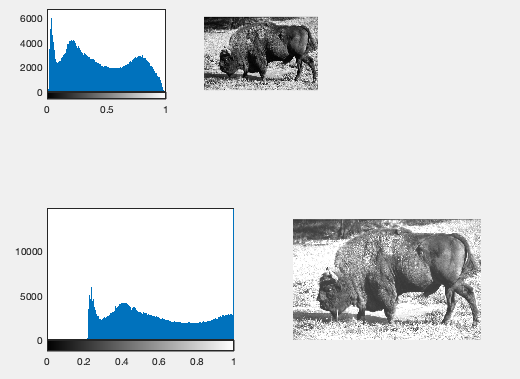
\includegraphics[width=18cm, height=16cm]{1}
\caption{Dodanie 0.2 do wartości pikseli}
\end{figure}

\paragraph{Odpowiednia manipulacja stałymi dodanymi / odjętymi od wszystkich pikseli zmienia nam jasność obrazu - odpowiednio dodając otrzymujemy obraz jaśniejszy, a odejmując ciemniejszy. Na histogramie natomiast widać przesunięcie całego wykresu - jest to spowodowane właśnie dodaniem stałej. Parametr powinien znajdować się w przedziale (-1, 1) - w innym wypadku odejmiemy / dodamy "za dużo" i przy sprowadzeniu obrazu do zakresu (0, 1) otrzymamy same zera lub same jedynki}

\subsection{Mnożenie wartości pikseli przez stałą - zmiana kontrastu}

\begin{figure}[h]
\centering
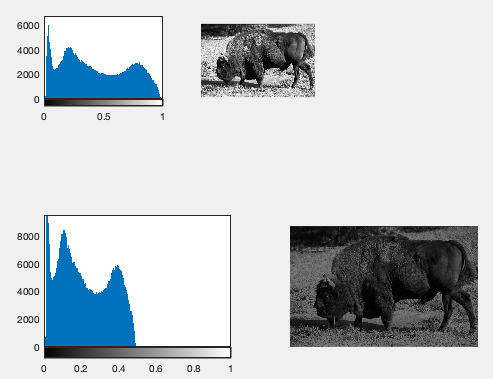
\includegraphics[width=18cm, height=16cm]{2}
\caption{Przemnożenie pikseli przez 0.5}
\end{figure}

\paragraph{Jak widać powyżej mnożenie powoduje zmianę kontrastu - w przypadku mnożenie przez liczbę większą od 1 uwydatnione zostaną jasne miejsca obrazu, natomiast poniżej jedynki uwydatnia ciemne fragmenty. Mnożenie przez 0 i liczby mniejsze oczywiście nie ma sensu - mnożenie przez 0 "usunęłoby" nam obraz - wszystkie piksele stałyby się zerami. Jak widać na histogramie zmienia nam się również zakres wartości pikseli. }

\subsection{Przesunięcie wybranego punktu do zera}

\begin{figure}[h]
\centering
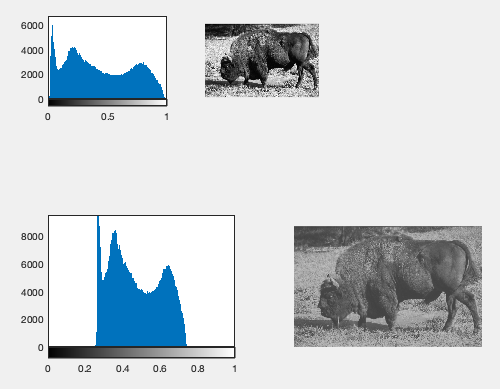
\includegraphics[width=18cm, height=16cm]{3}
\caption{Przesunięcie pikseli o 0.5 i przemnożenie przez 0.5}
\end{figure}

\paragraph{Przesuwamy wybrany punkt "do 0" -> przemnożony przez każdą stałą będzie dalej równy zero. }

\subsection{Potęgowanie wartości pikseli przez stałą - zmiana parametru gamma}

\begin{figure}[h!]
\centering
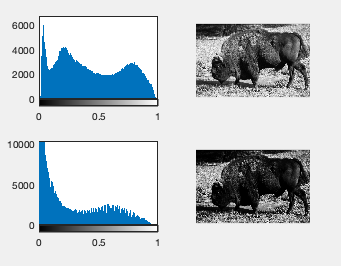
\includegraphics[width=18cm, height=16cm]{4}
\caption{Podniesienie pikseli do drugiej potęgi}
\end{figure}

\paragraph{W czasie potęgowania parametr $G$ zwykle jest równy odwrotności, aby zgodnie z intuicją mniejsze wartości dawały jaśniejszy obraz - gdy potęgujemy przez stałą z przedziału (0; 1) obraz ulega rozjaśnieniu. W przeciwnym wypadku obraz zostanie zaciemniony. Efekt jednak tym razem będzie nieliniowy co pozwala nam uniknąć przepaleń na obrazie oraz osiągnąć jednolite rozmycie. }

\newpage

\section{Laboratoria 3}

\paragraph{Na trzecich zajęciach natomiast nauczyliśmy się korzystać z różnego rodzaju filtrów przy pomocy funkcji $imfilter$, $imerode$, $mdefilt2$, $fspecial$, $imdilate$, oraz przy pomocy funkcji, które pomagały nam przy przygotowaniu obrazu do filtracji: $imbinarize$, $graythresh$}

\subsection{Filtr górnoprzepustowy}

\begin{figure}[h!]
\centering
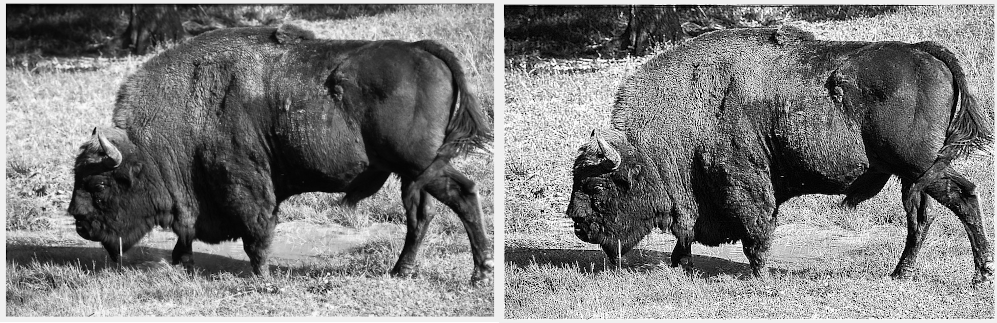
\includegraphics[width=18cm, height=8cm]{5}
\caption{Filtr górnoprzepustowy}
\end{figure}

\newpage

\paragraph{Efekt: Uwydatnione krawędzie}

\subsection{Filtr dolnoprzepustowy}

\begin{figure}[h!]
\centering
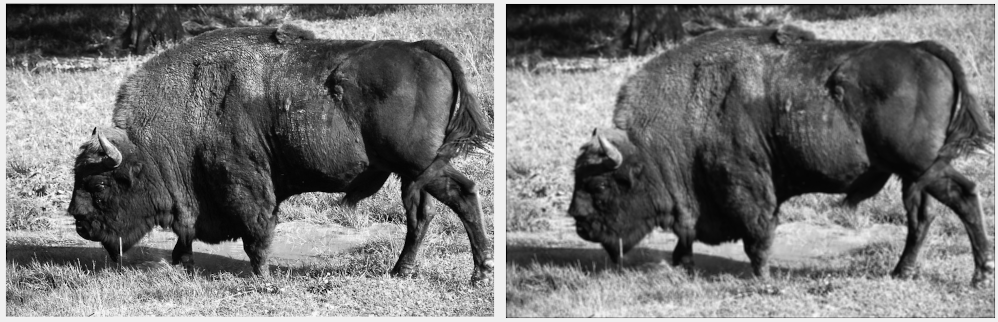
\includegraphics[width=18cm, height=8cm]{6}
\caption{Filtr dolnoprzepustowy}
\end{figure}

\paragraph{Efekt: Usuwanie dużych różnic na obrazie pomiędzy kolorami}

\newpage

\subsection{Filtr medianowy}

\begin{figure}[h!]
\centering
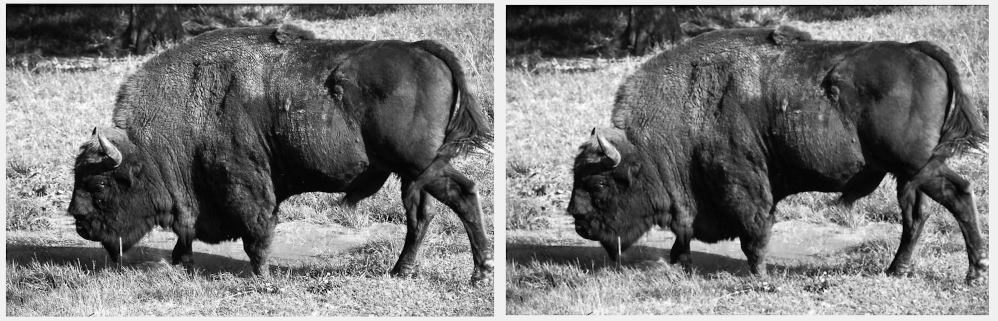
\includegraphics[width=18cm, height=8cm]{7}
\caption{Filtr medianowy}
\end{figure}

\paragraph{Efekt: Podobny jak poprzednio, jednak odszumia jedynie porządane elementy obrazu, nie zaburza reszty sygnału.}

\newpage

\subsection{Filtr "prewitt"}

\begin{figure}[h!]
\centering
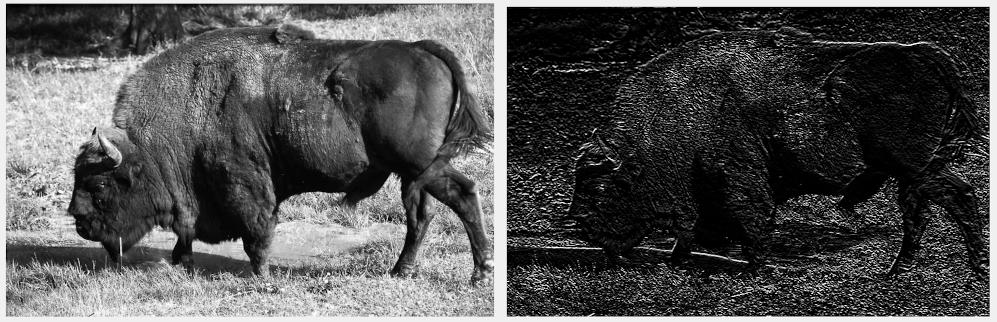
\includegraphics[width=18cm, height=8cm]{8}
\caption{Filtr "prewitt"}
\end{figure}

\paragraph{Wykorzystywany do wykrywania krawędzi - głównie poziomych}

\newpage

\subsection{Filtr "sobel"}

\begin{figure}[h!]
\centering
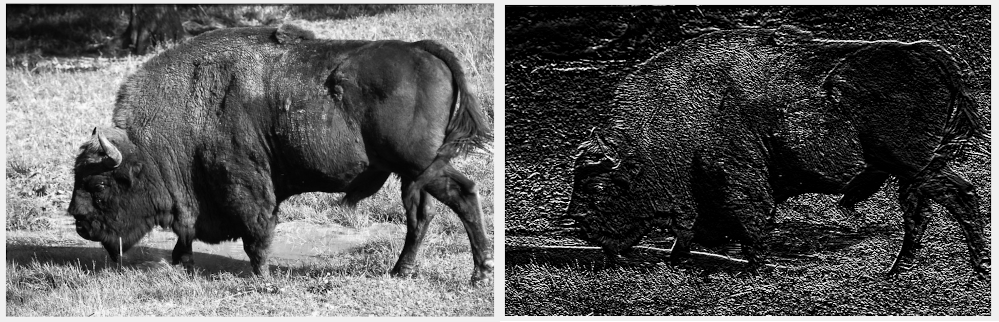
\includegraphics[width=18cm, height=8cm]{9}
\caption{Filtr "sobel"}
\end{figure}

\paragraph{Wykorzystywany do wykrywania krawędzi - głównie poziomych}

\newpage

\subsection{Binaryzacja obrazu}

\begin{figure}[h!]
\centering
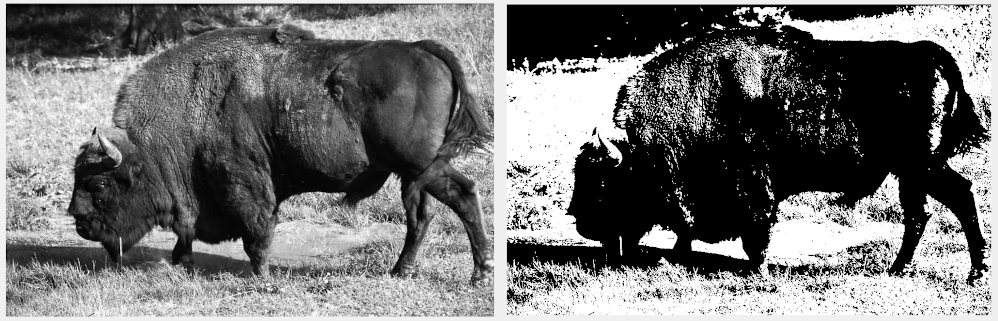
\includegraphics[width=18cm, height=8cm]{10}
\caption{Binaryzacja obrazu}
\end{figure}

\paragraph{Na podstawie binaryzacji w tym przypadku możemy na przykład oddzielić żubra od tła. Po binaryzacji, nasze piksele przyjmują tylko wartości 0 lub 1.}

\newpage

\subsection{Erozja}

\begin{figure}[h!]
\centering
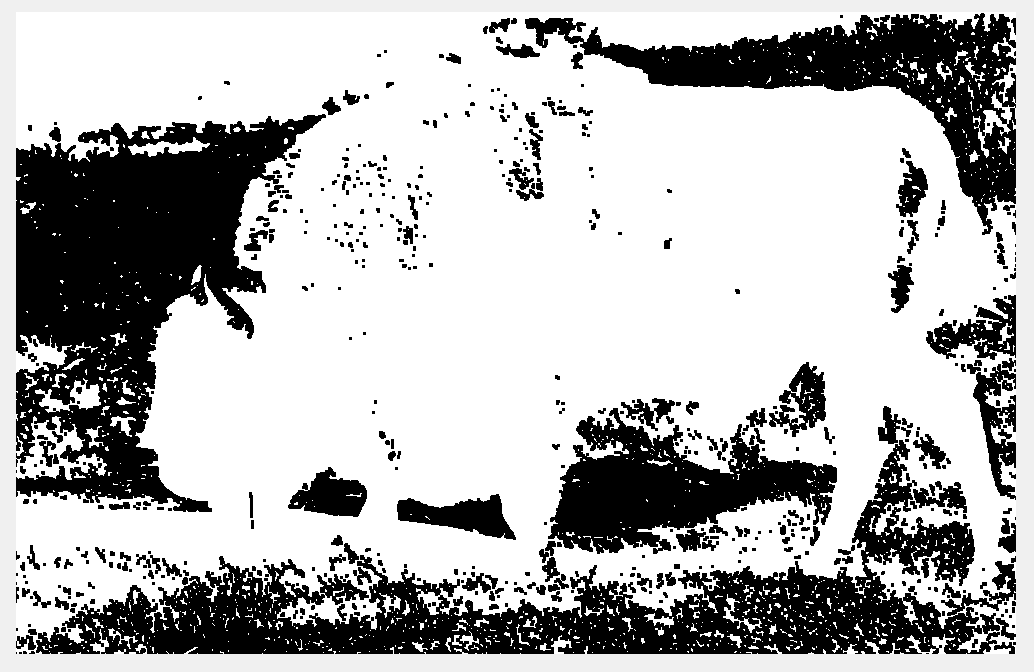
\includegraphics[width=12cm, height=6cm]{11}
\caption{Erozja}
\end{figure}

\paragraph{Efekt: Pomniejsza krawędzie na obrazie, dokonuje zmian, gdy w sąsiedztwie jasnego piksela znajdują się ciemne (chociaż jeden).}

\newpage

\subsection{Dylatacja}

\subsection{Erozja}

\begin{figure}[h!]
\centering
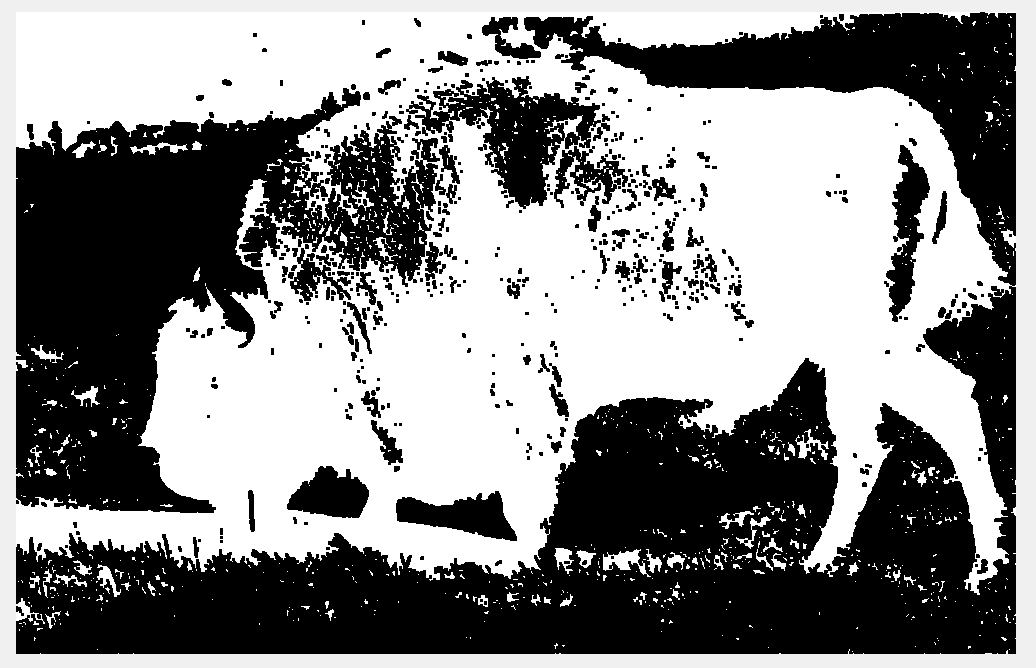
\includegraphics[width=12cm, height=6cm]{12}
\caption{Dylatacja}
\end{figure}

\paragraph{Efekt: Powiększa krawędzie na obrazie, dokonuje zmian, gdy w sąsiedztwie ciemnego piksela znajdują się jasne (chociaż jeden).}

\newpage

\subsection{Dylatacja + Erozja - otwarcie}

\begin{figure}[h!]
\centering
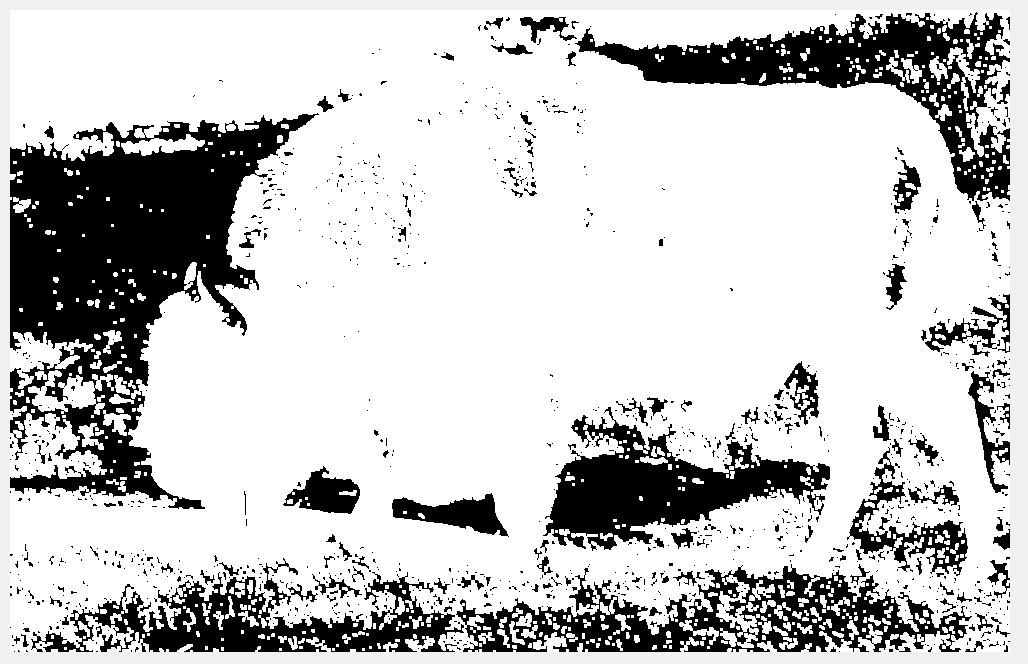
\includegraphics[width=12cm, height=6cm]{13}
\caption{Otwarcie}
\end{figure}

\paragraph{Efekt: Małe jasne punkty znikają, natomiast ciemne punkty wyglądają podobnie.}

\newpage

\subsection{Erozja + Dylatacja - zamknięcie}

\begin{figure}[h!]
\centering
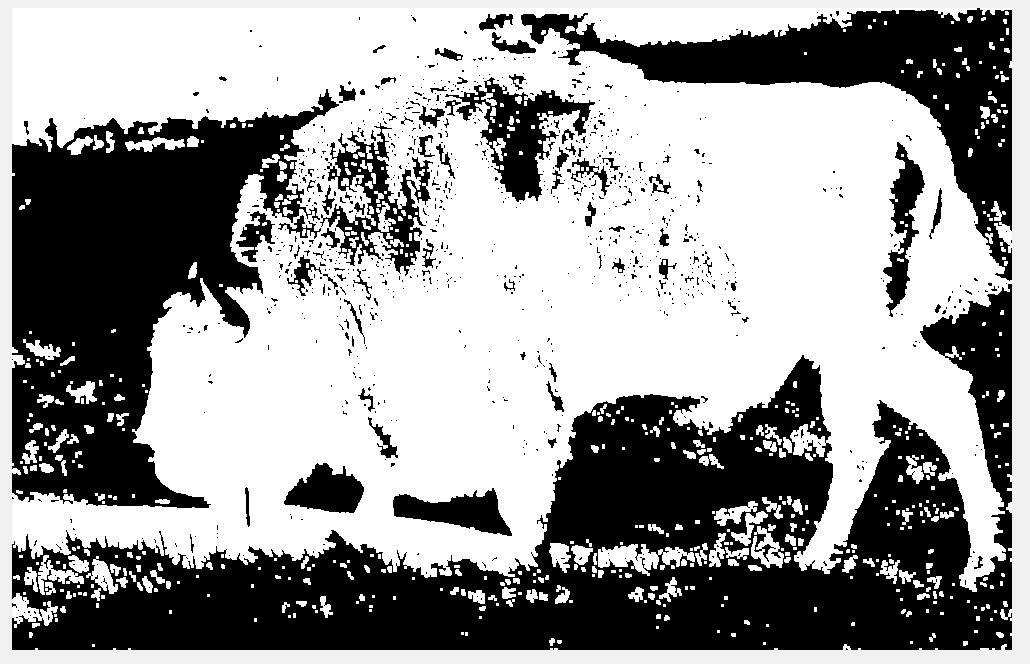
\includegraphics[width=12cm, height=6cm]{14}
\caption{Zamknięcie}
\end{figure}

\paragraph{Efekt: Małe ciemne punkty znikają, natomiast jasne są podobne.}

\newpage

\section{Laboratoria 4}

\paragraph{Na czwartych laboratoriach wykorzystywaliśmy transformatę Fourier'a w celu dokonywania zmian na obrazach oraz filtracji. Dzięki środowisku Matlab i funkcjom $fftshift$ oraz $fft2$ ("Fast Fourier Transform 2") nie musieliśmy sami implementować tychże funkcjonalności.}

\paragraph{Korzystająć z tranformaty Fourier'a możemy dokonywać również filtracji - tak jak na przykładzie na samym końcu - dokonaliśmy rozmycia oraz inwersji.}

\newpage

\begin{figure}[h!]
\centering
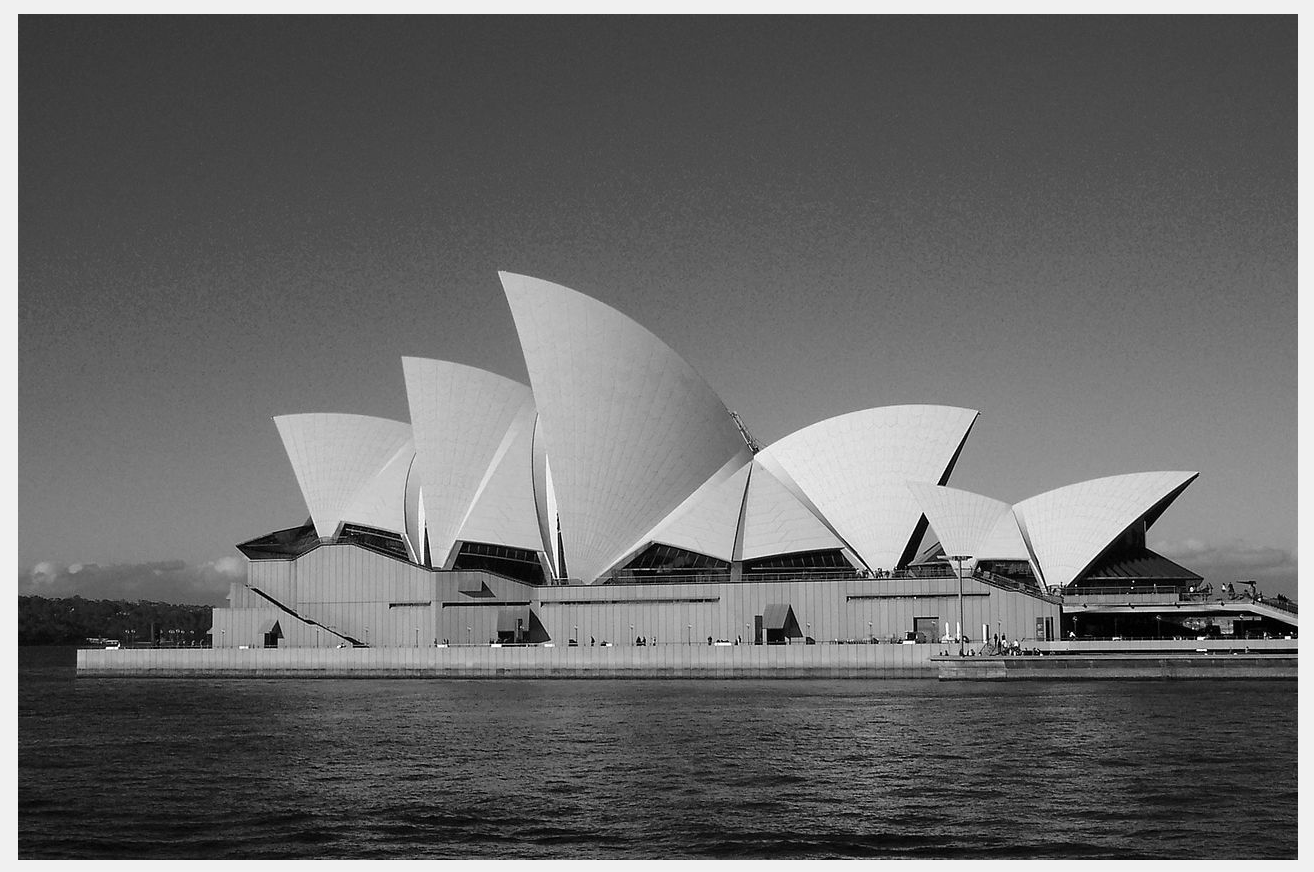
\includegraphics[width=18cm, height=12cm]{sydney}
\caption{Obraz oryginalny}
\end{figure}

\newpage

\begin{figure}[h!]
\centering
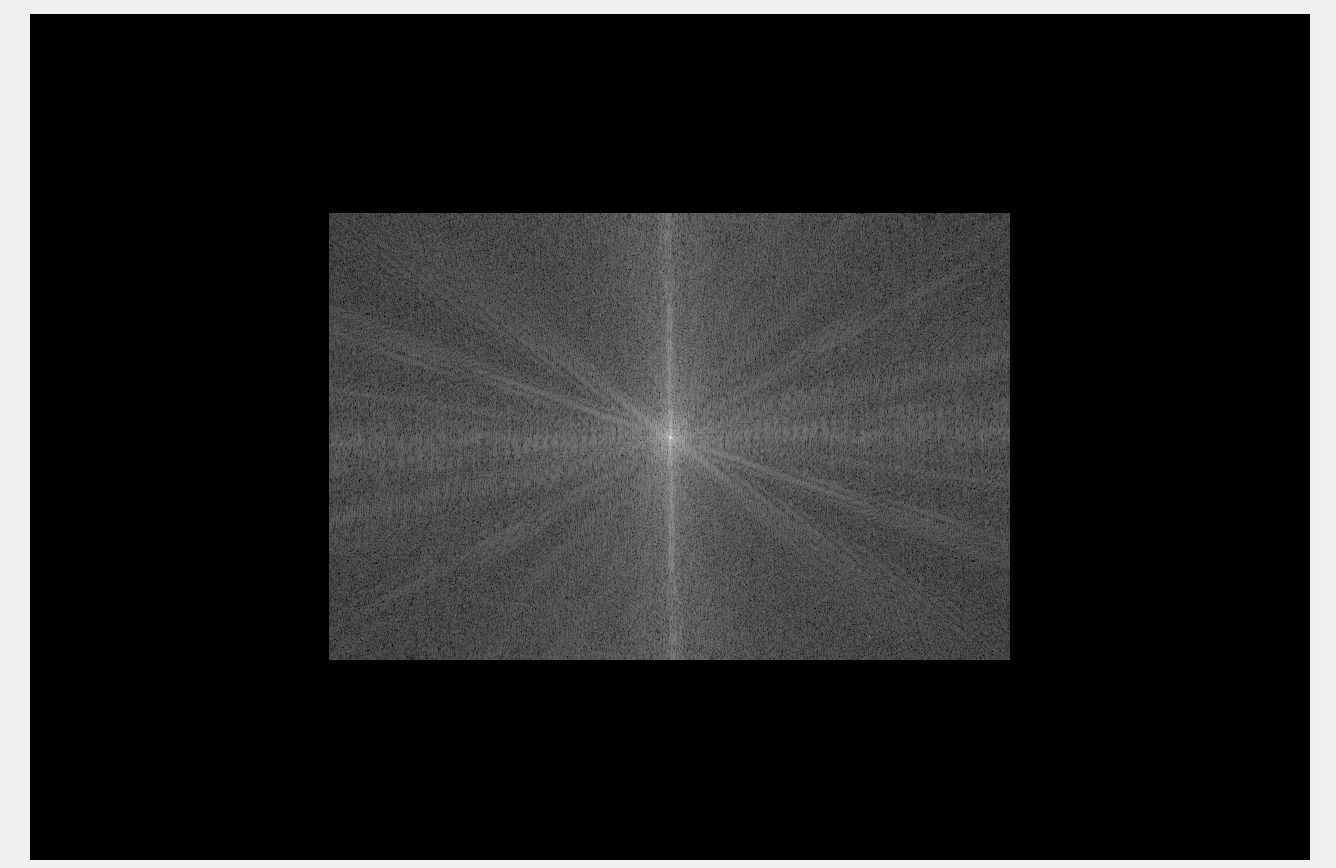
\includegraphics[width=18cm, height=12cm]{widmo_ampl}
\caption{Widmo amplitudowe obrazu}
\end{figure}

\newpage

\begin{figure}[h!]
\centering
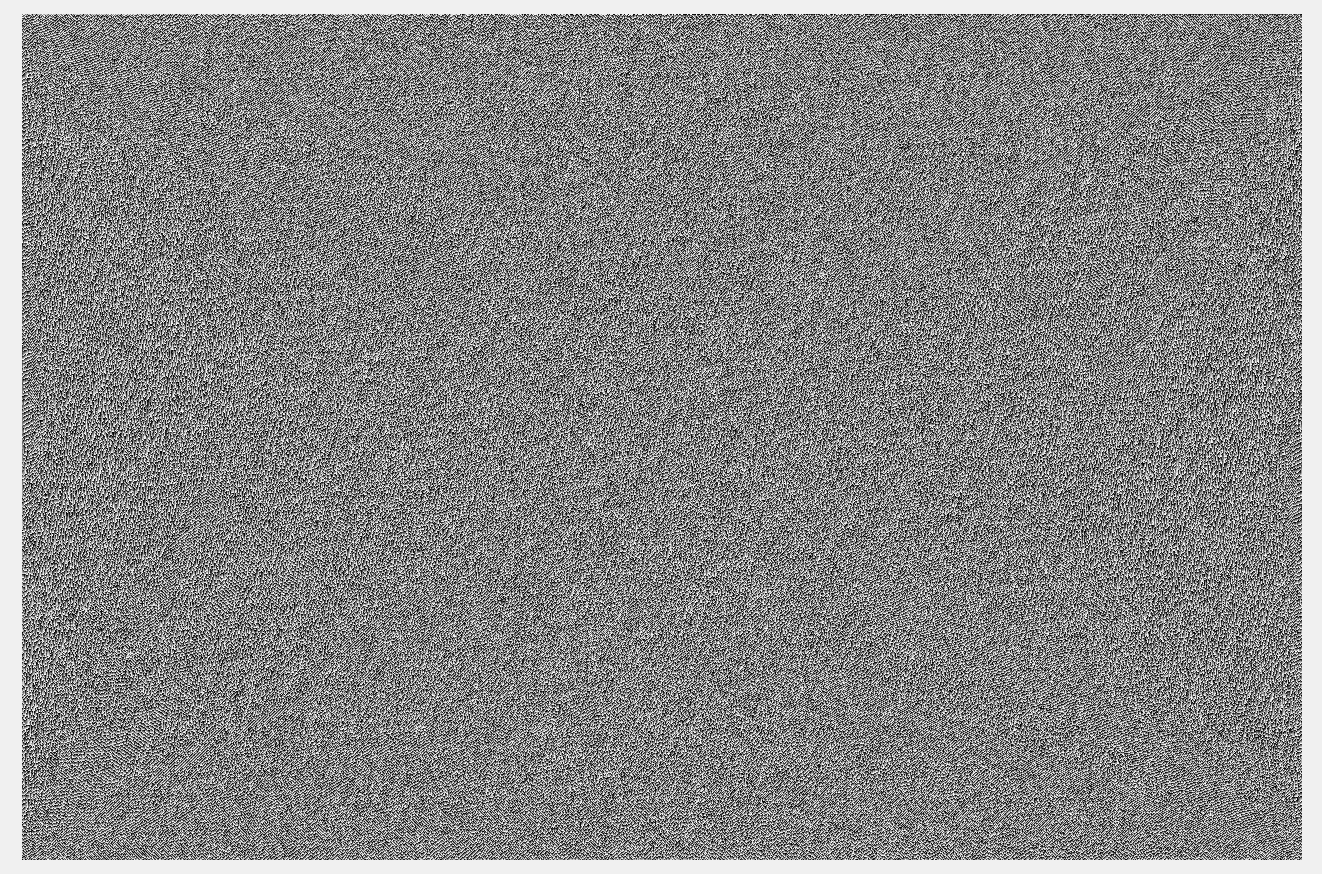
\includegraphics[width=18cm, height=12cm]{widmo_faz}
\caption{Widmo fazowe obrazu}
\end{figure}

\newpage

\begin{figure}[h!]
\centering
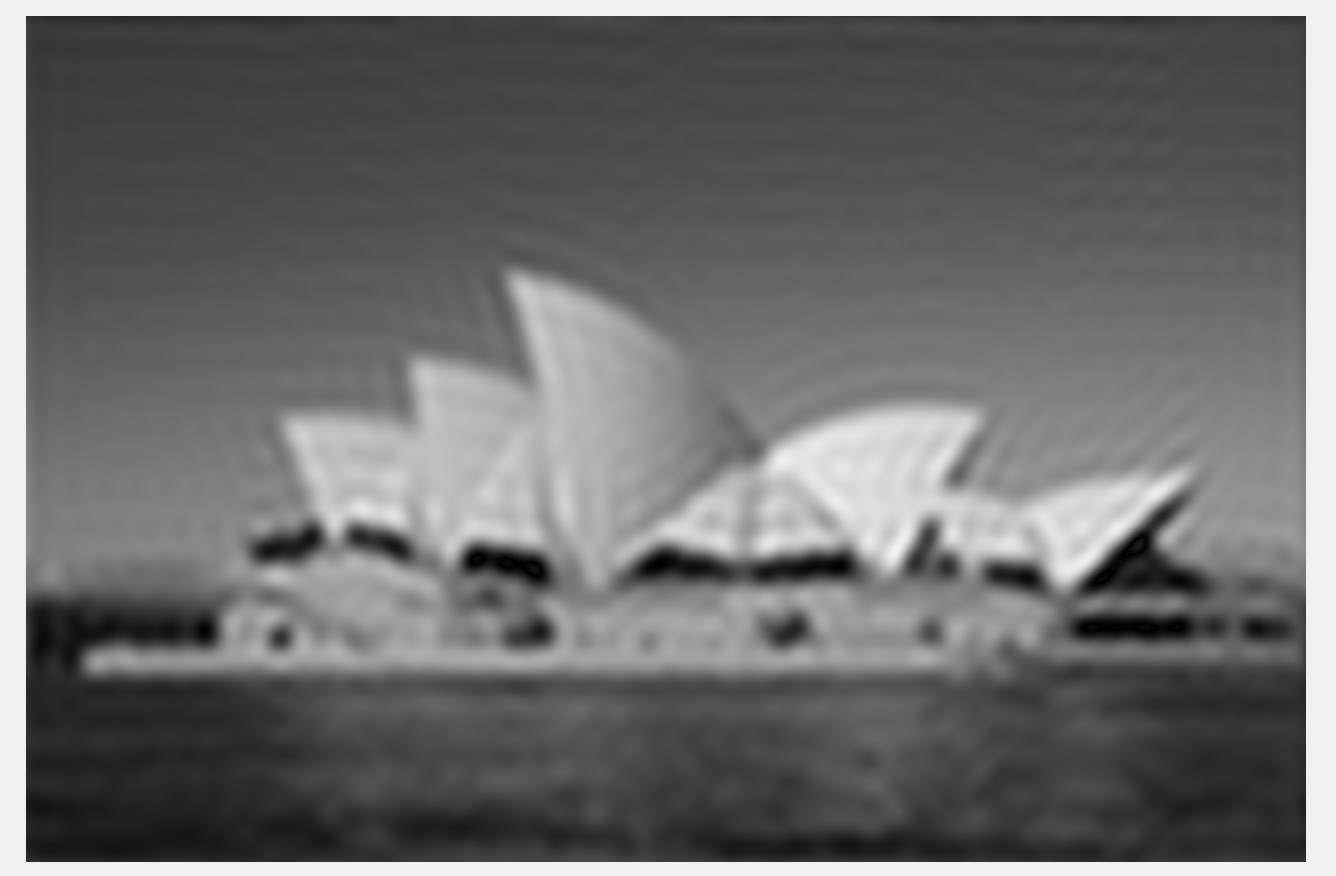
\includegraphics[width=18cm, height=12cm]{rozmycie}
\caption{Dodanie maski - rozmycie Gauss'a}
\end{figure}

\newpage

\begin{figure}[h!]
\centering
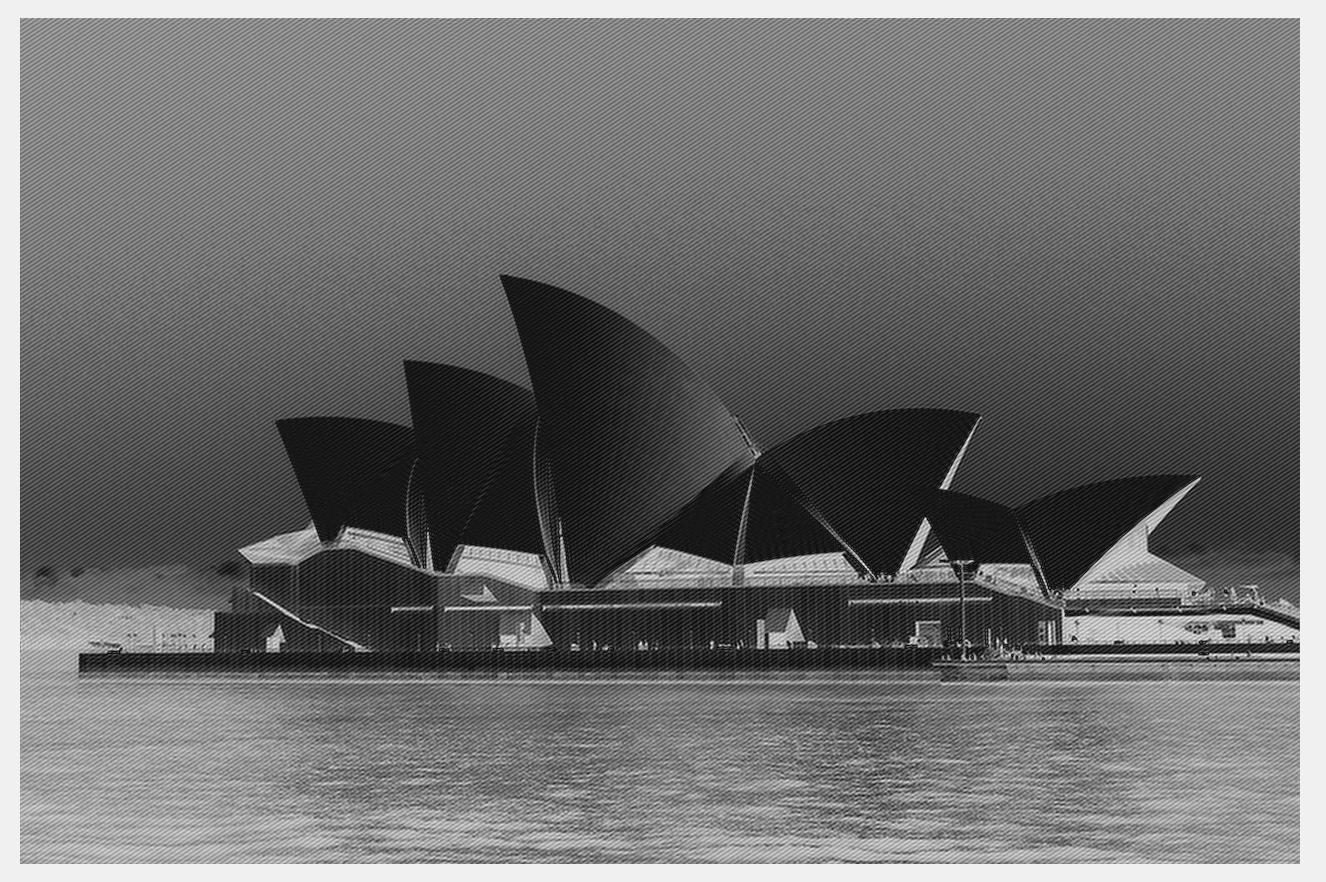
\includegraphics[width=18cm, height=12cm]{inwersja}
\caption{Zmiana fazy - inwersja obrazu + maski - kompresja}
\end{figure}

\end{justify}
\end{document}